%% ============================================================
%% SECTION*: Part II — Comprehensive Architecture of the Proposed Framework
%% ============================================================

\section*{Part II: Comprehensive Architecture of the Proposed Framework}

The dataflow in the architecture follows a structured top-down and bottom-up autoencoder progression, enabling hierarchical feature extraction, contextual integration, and precise voxel-wise reconstruction. The input data is fed to the encoder side and the segmented output is received from the decoder side.
The data flow through the architecture can be understood by tracing the processing pipeline from the raw BraTS data to the final segmentation map. to the final segmentation map.

\subsection{Input Preprocessing and Normalization}

The raw input data (.nii files) are passed through a custom data generator that stacks 3 of the 4 channels belonging to an input data into a NumPy array of size $128 \times 128 \times 128 \times 3$.
Each subject is represented as a pre-aligned multi-modal MRI volume:
$X_0 = \{X^{(1)} X^{(2)} X^{(3)} X^{(4)}\} - \{X^{(1)}\}\in \mathbb{R}^{(H\times W\times D\times 3)}$, where $X^{(1)}, X^{(2)}, X^{(3)}, X^{(4)}$ correspond to the T1, T1ce, T2, and FLAIR modalities respectively, and $H = W = D = 128$. Before entering the network, each modality is min-max normalized independently to [0, 1]. The three channels are stacked to form the initial 3D input tensor in the form of a NumPy array converted from the .nii file format. The height, width, and depth of 128 is achieved by hard cropping into the middle of the middle where most of the data resides, discarding the empty space outside the relevant brain area.

\begin{figure*}[!htbp]
    \centering
    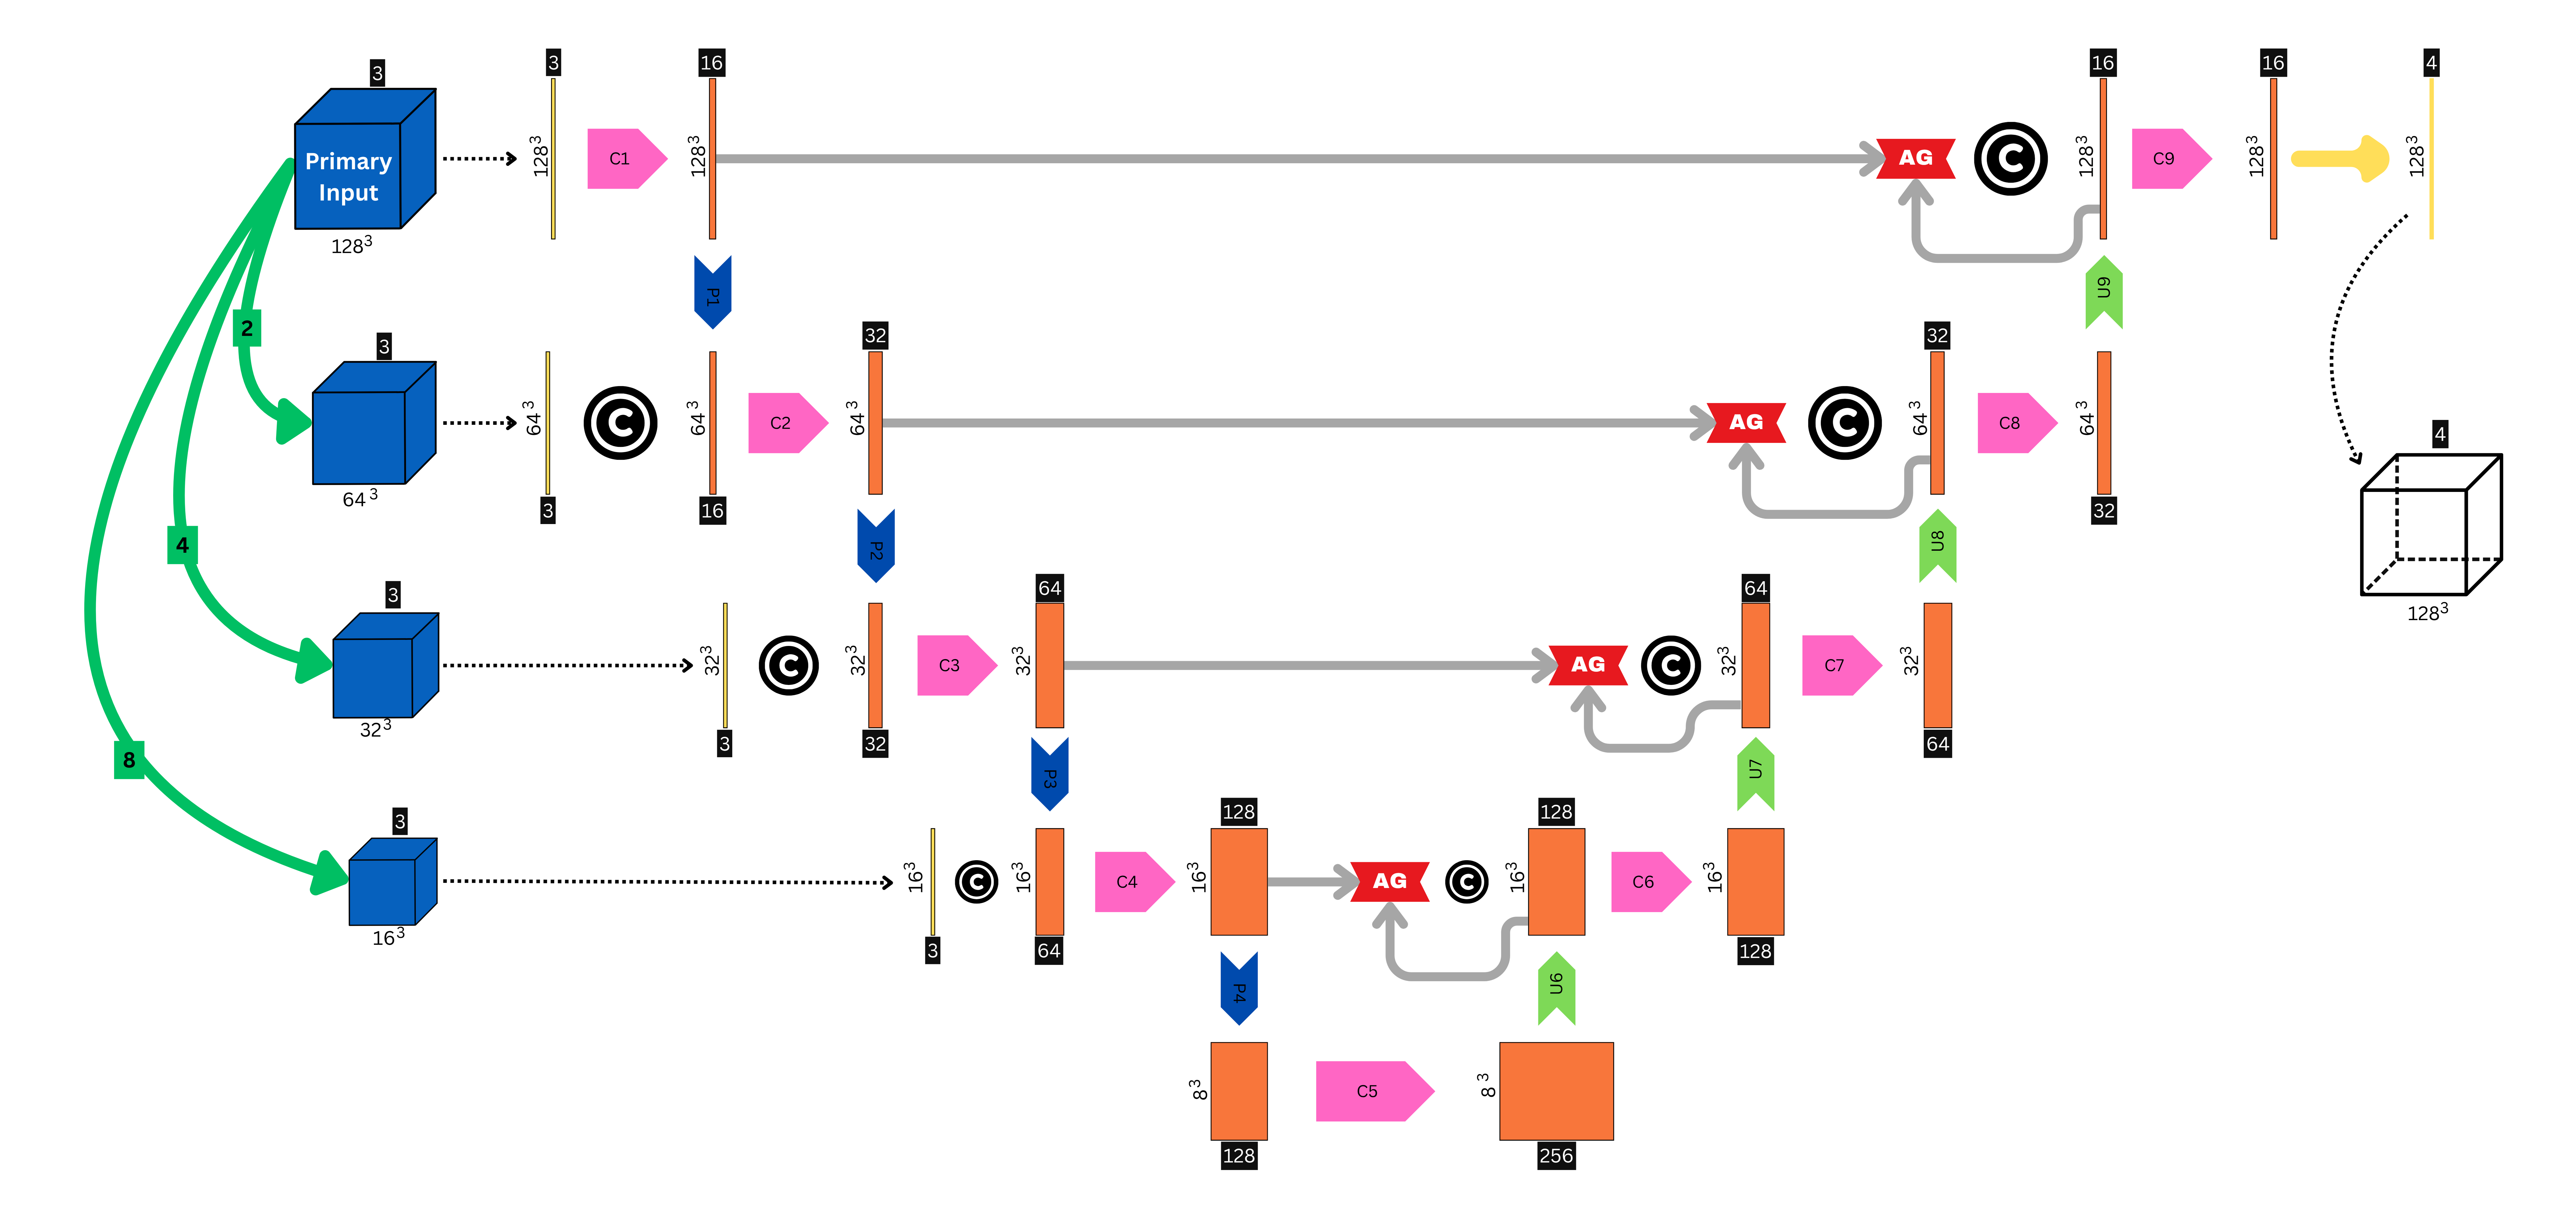
\includegraphics[width=\textwidth]{figs/Overall Architecture.png}

    \vspace{2mm}

    \setlength{\dashlinedash}{0.5pt}
    \setlength{\dashlinegap}{1.5pt}

    \fbox{
    \begin{tabular}{cl|cl|cl}

    
\includegraphics[width=0.018\textwidth]{figs/Label1/1.png}
    & \scriptsize Concatenation
    &
    
\includegraphics[width=0.015\textwidth]{figs/Label1/9.png}
    & \scriptsize MaxPool
    &
    
\includegraphics[width=0.015\textwidth]{figs/Label1/7.png}
    & \scriptsize TransConv

    \\[1.5mm]
    \hdashline

    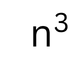
\includegraphics[width=0.030\textwidth]{figs/Label1/3.png}
    & \scriptsize Dimension
    &
    
\includegraphics[width=0.030\textwidth]{figs/Label1/4.png}
    & \scriptsize Number of channels
    &
    
\includegraphics[width=0.030\textwidth]{figs/Label1/8.png}
    & \scriptsize Dense Inception-Res Block

    \\[1.5mm]
    \hdashline

    
\includegraphics[width=0.030\textwidth]{figs/Label1/10.png}
    & \scriptsize AttentionGate
    &
    
\includegraphics[width=0.030\textwidth]{figs/Label1/2.png}
    & \scriptsize Average-pooled by factor of $n$
    &
    
\includegraphics[width=0.030\textwidth]{figs/Label1/11.png}
    & \scriptsize Conc 1x1x1 with sigmoid

    \\

    \end{tabular}
    }

    \caption{Integrated Architectural Framework}
    \label{FIG:Overall Architecture}
\end{figure*}

\subsection{Encoder (Contracting Path)}

At each encoder stage $l\in\{1,2,3,4\}$, the network performs three sequential operations:
\begin{itemize}
    \item Feature Extraction (Dense Inception Residual Convolution):
    \begin{itemize}
        \item Each stage applies a DRIC block, combining multiple convolutional branches with different receptive fields
        \item The block output is: $F_l = DRIC_l (X_{l-1})$
    \end{itemize}
    \item Downsampling:
    \begin{itemize}
        \item The feature map is halved in each spatial dimension using 3D max pooling: $X_l = MaxPool3D(F_l,\allowbreak\, p = 2)$, where $p$ represents the scaling factor.
    \end{itemize}
    \item Skip Connection Storage:
    \begin{itemize}
        \item Each pre-pooled feature map $F_l$ is preserved for later fusion with the decoder at the corresponding level.
    \end{itemize}
\end{itemize}

\subsection{Multiscale Input}

The input in the form of numpy array is downsampled through an simple average pooling function that converts the primary input of size $128^3\times3$ into multiple scaled down inputs of $128^3\times3$, $64^3\times3$, and $32^3\times3$; that is then fed to the encoder at different stages.
The original input $X_0$ (of size $128^3\times3$) is successively downsampled:
$\tilde{X}_l=Downsample(X_0,scale=2^l), l$ represents the encoder stage, and concatenated with $X_{l-1}$ before entering the next DRIC block:
$\hat{X}_l=[X_{l-1} \| \tilde{X}_l]$.

\subsection{Bottleneck (Bridge)}

The lowest-level encoder output passes through a bottleneck DRIC block, $B = DRIC_{bottleneck}(X_4)$.

\subsection{Decoder (Expanding Path)}

The decoder path performs progressive upsampling and reconstruction to return the segmentation to full spatial resolution. At each decoder stage $m \in {4,3,2,1}:$

\begin{itemize}
    \item Upsampling:
The feature map is expanded using transposed 3D convolutions: $U_m = ConvTranspose3D\allowbreak(B_m, k = 2, s = 2)$, where $k$ and $s$ denote kernel size and stride, respectively.
\end{itemize}

\begin{itemize}
    \item Attention-Gated Skip Connection:
Before concatenating with its encoder counterpart $F_m$, an attention gate filters the encoder feature map based on relevance to the decoder's context.
Let the gating signal of the decoder be $g_m$ and the encoder feature be $F_m$; the attention coefficient is computed as:
$\alpha_m = \sigma(W_g * g_m + W_x * F_m+b),$ and the refined feature map is: $\tilde{F}_m=\alpha_m \odot F_m,$ where $\odot$ denotes element-wise multiplication. This suppresses irrelevant background and enhances focus on tumor boundaries and salient regions.
\end{itemize}

\begin{itemize}
    \item Fusion and Convolution:
		The attention-refined skip feature $\tilde{F}_mis$ concatenated with $U_m:
    \\C_m=[U_m \| \tilde{F}_m],$ which is then processed by another DRIC block: $B_{m-1} = DRIC_m(C_m)$.
\end{itemize}

\subsection{Output Layer}

After the final decoder stage, a $1 \times 1 \times 1$ convolution projects the feature volume into the four output classes: $Y=Softmax(W_{out} * B_0 + b_{out})$,
where $Y \in [0,1]^{H \times W \times D \times 4}$ represents per-voxel class probabilities for background, NCR/NET, ED, and ET.
